\chapter{前端架構}
\section{技術介紹}

前端-在此為 Android 手機-負責了 AR 場景的繪製。這部分藉助了由 Google 所提供的 \href{https://developers.google.com/ar}{ARCore}\footnote{\url{https://developers.google.com/ar}},對圖 \ref{fig:標定物} 進行姿態估計與使用 OpenGL ES 繪製 3D 物件於場景中。

\begin{figure}[h]
    \centering
    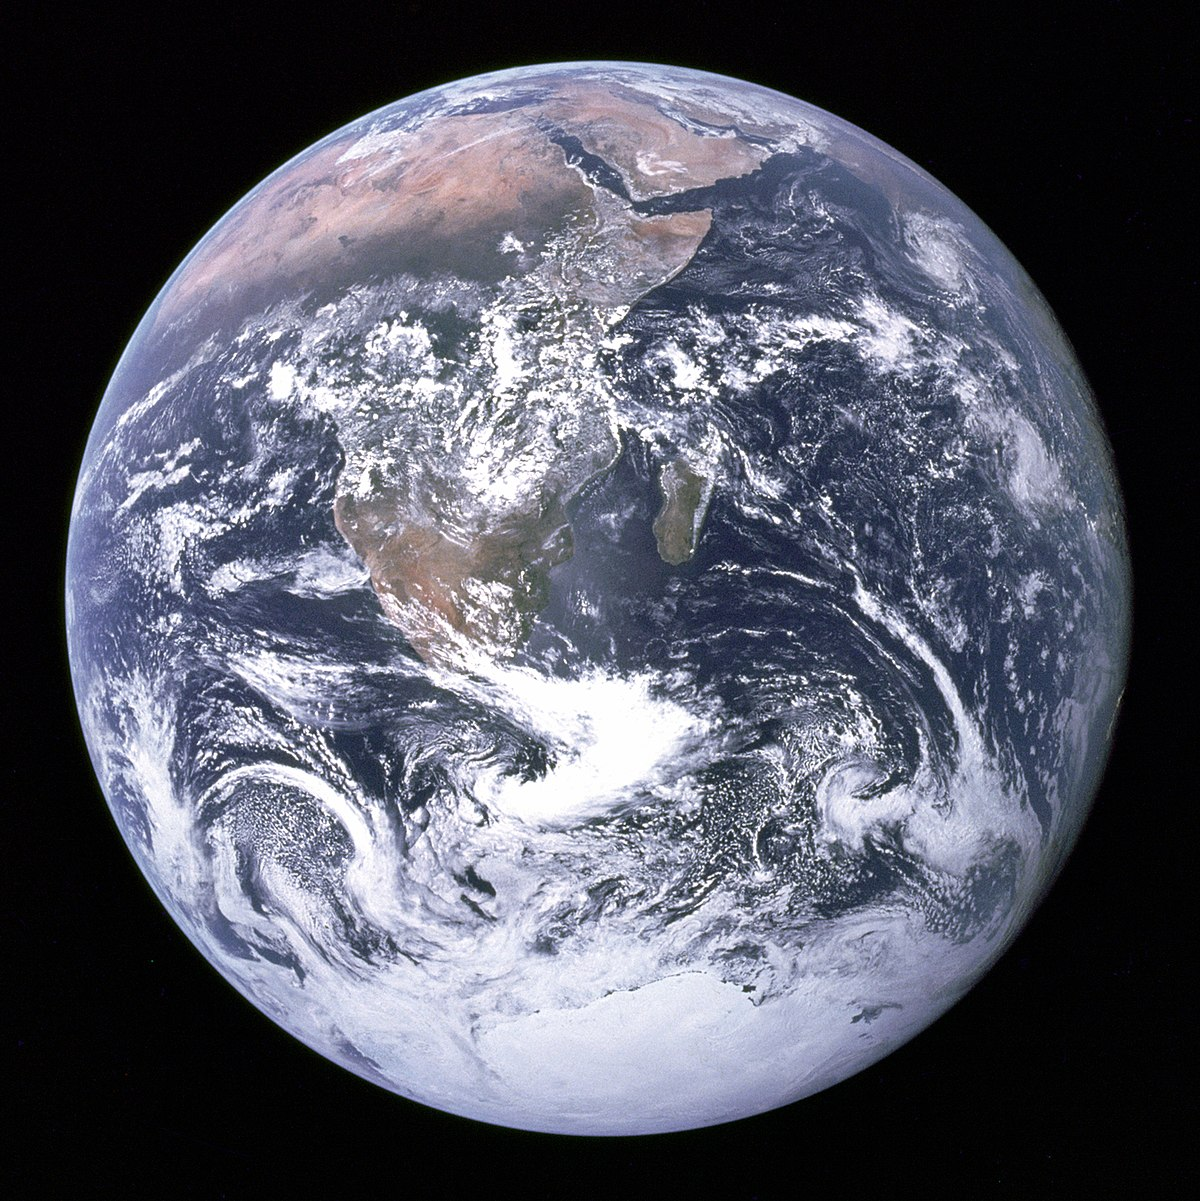
\includegraphics[width=3cm]{mark.jpg}
    \caption{標定物}
    \label{fig:標定物}
\end{figure}

\section{技術說明與實作}
\subsection{ARCore 姿態估計}
\subsubsection{安裝}

欲使用 ARCore 必須先安裝 Google 所提供的應用程式,該應用程式可以在 \href{https://play.google.com/store/apps/details?id=com.google.ar.core}{Google Play}\footnote{\url{https://play.google.com/store/apps/details?id=com.google.ar.core}} 上找到。須注意並非所有 Android 裝置都支援這個應用程式,支援的裝置列表可以在\href{https://developers.google.com/ar/discover/supported-devices#google_play_device}{此處}\footnote{\url{https://developers.google.com/ar/discover/supported-devices\#google\_play\_device}}查詢。

\subsubsection{準備、初始化}

在安裝後需要撰寫一系列繁雜且固定的初始化流程,才能在執行期安全地取得讓我們能夠使用 ARCore 的物件-com.google.ar.core.Session-這一系列的繁雜任務不多做贅述,可以於\href{https://developers.google.com/ar/develop/java/enable-arcore}{此處}\footnote{\url{https://developers.google.com/ar/develop/java/enable-arcore}}查看。

\subsubsection{標定物設定}

為了使標定物能夠被 ARCore 偵測,使用了 \href{https://developers.google.com/ar/develop/java/augmented-images}{Augmented Images}\footnote{\url{https://developers.google.com/ar/develop/java/augmented-images}} 相關的 API。需要先將影像加入 \href{https://developers.google.com/ar/reference/java/com/google/ar/core/AugmentedImageDatabase}{AugmentedImageDatabase}\footnote{\url{https://developers.google.com/ar/reference/java/com/google/ar/core/AugmentedImageDatabase}},之後將該物件交給 \href{https://developers.google.com/ar/reference/java/com/google/ar/core/Session}{Session}\footnote{\url{https://developers.google.com/ar/reference/java/com/google/ar/core/Session}}。具體有二種做法。

於執行時將圖片動態載入 AugmentedImageDatabase:

\begin{lstlisting}[language=Java, caption=動態載入圖片]
InputStream is = getAssets().open("image.png")
Bitmap augmentedImageBitmap = BitmapFactory.decodeStream(is)

AugmentedImageDatabase augmentedImageDatabase;
augmentedImageDatabase = new AugmentedImageDatabase(session);
augmentedImageDatabase.addImage("image", 
                                augmentedImageBitmap,
                                /*widthInMeters = */0.25f);

Config config = new Config(session);
config.setAugmentedImageDatabase(augmentedImageDatabase);
session.configure(config);
\end{lstlisting}

或是預先使用 \href{https://developers.google.com/ar/develop/java/augmented-images/arcoreimg}{arcoreimg tool}\footnote{\url{https://developers.google.com/ar/develop/java/augmented-images/arcoreimg}} 將圖片(可多張)打包成 AugmentedImageDatabase 可讀取的 *.imgdb 檔案

\begin{lstlisting}[language=bash, caption=使用 arcoreimg tool 將圖片打包]
arcoreimg.exe build-db --input_image_list_path=/path/to/image_list_file.txt --output_db_path=/path/to/myimages.imgdb
\end{lstlisting}

image\_list\_file.txt 格式為:以 | 分隔,順序為圖片名稱、圖片位置、圖片物理寬度(公尺,非必要,有助於 ARCore 偵測圖片)。

\begin{lstlisting}[caption=image\_list\_file.txt 範例]
mouse|path/to/mouse.png|0.1
little dog|/path/to/dog.jpg
\end{lstlisting}

之後便可將 myimages.imgdb 交給 Session

\begin{lstlisting}[language=Java, caption=將 myimages.imgdb 交給 Session]
AugmentedImageDatabase augmentedImageDatabase;
InputStream is = getAssets().open("myimages.imgdb")
augmentedImageDatabase = AugmentedImageDatabase.deserialize(session, is);

Config config = new Config(session);
config.setAugmentedImageDatabase(augmentedImageDatabase);
session.configure(config);
\end{lstlisting}

\subsubsection{偵測標定物}
將 AugmentedImageDatabase 透過 Config 設定給 Session 後,便可透過 \lstinline{session.update()} 更新 Augmented Image 的追蹤情形。

\begin{lstlisting}[language=Java, caption=取得影像追蹤狀態]
Frame frame = session.update();
Collection<AugmentedImage> updatedAugmentedImages = frame.getUpdatedTrackables(AugmentedImage.class);

for (AugmentedImage augmentedImage : updatedAugmentedImages) {
    switch (augmentedImage.getTrackingState()) {
        case PAUSED:
            // When an image is in PAUSED state, but the camera is not PAUSED, it has been detected, but not yet tracked.
            break;

        case TRACKING:
            // The Trackable is currently tracked and its pose is current.
            break;

        case STOPPED:
            // ARCore has stopped tracking this Trackable and will never resume tracking it.
            break;

        default:
            break;
}
\end{lstlisting}

\subsubsection{取得標定物姿態}

在 Tracking 狀態下,可透過 \lstinline{augmentedImage.getCenterPose()} 取得 Augmented Image 在世界坐標系(該坐標系由 ARCore 管理)的姿態(未 Tracking 時會是上一次 Tracking 的最後位置),該姿態 +X 軸從影像左側指向右側, +Z 軸從影像上側指向下側,+Y 軸指出該平面。

\subsection{OpenGL 物件位置與實景貼合}

透過 OpenGL 繪製物件需透過三個 Matrix 完成座標點的轉換:分別為 Projection, View, Model

\subsubsection{Model Matrix}
將位於 Model coordinate 的座標點轉移至 World coordinate

\subsubsection{View}
將位於 World coordinate 的座標點轉移至 Camera coordinate

\subsubsection{Projection}
將位於 Camera coordinate 的座標點轉移至 Clip coordinate。

\begin{center}
    $
        coordinate\_in\_clip = Projection\_Matrix \times View\_Matrix \times Model\_Matrix \times model\_coordinate
    $
\end{center}

這些矩陣皆可透過 ARCore 取得,僅需注意其順序為 Column-major。

\subsubsection{取得 Model Matrix}

Model matrix 可以由藉由追蹤中物件取得,例如想取得將 3D Model 轉移至標定物姿態的矩陣。

\begin{lstlisting}[language=Java, caption=將 3D model 的座標空間轉移至以標定物為準的空間]
Frame frame = session.update();
Collection<AugmentedImage> updatedAugmentedImages = frame.getUpdatedTrackables(AugmentedImage.class);

// Assume only one image
AugmentedImage augmentedImage = updatedAugmentedImages.iterator().next();

float[] modelMatrix = new float[16];
switch (augmentedImage.getTrackingState()) {
    case TRACKING:
        augmentedImage.getCenterPose().toMatrix(modelMatrix, /*offset = */ 0);
        break;

    default:
        break;
}
\end{lstlisting}

\subsubsection{取得 View Matrix}

相機坐標系的管理由 ARCore 掌握,若想取得 View Matrix。

\begin{lstlisting}[language=Java, caption=取得 View Matrix]
Frame frame = session.update();
Camera camera = frame.getCamera();

float[] viewMatrix = new float[16];
camera.getViewMatrix(viewMatrix, /*offset = */ 0);
\end{lstlisting}

\subsubsection{取得 Projection Matrix}

投影矩陣做法也類似。

\begin{lstlisting}[language=Java, caption=取得 Projection Matrix]
float[] projMatrix = new float[16];
camera.getProjectionMatrix(projMatrix,
/*offset = */ 0, /*near clipping plane = */ 0.01f, /*far clipping plane = */ 15.0f);
\end{lstlisting}

\subsubsection{OpenGL ES on Android}

Android SDK 包含了讓開發人員可以快速使用 OpenGL ES 的 API,舉體使用步驟為:

\begin{enumerate}
    \item 在 Manifest.xml 宣告使用 OpenGL ES
    \item 新增 android.opengl.GLSurfaceView 於畫面中(將該實例稱為 V)
    \item 繼承 android.opengl.GLSurfaceView,並將 V 指派給該 class。(可選,需要管理該 View 的 Touch event 才需要)
    \item 繼承 GLSurfaceView.Render 並實作(將該實例稱為 R)
    \item 將該 V 的 Render 設定為 R
\end{enumerate}


\subsection{遊戲設計}

\subsubsection{飛鏢動畫}

飛鏢動畫是依照射出的初速以及手機的初始位置製作的物件,可以依照飛行時間計算飛鏢當下的鋼體參數。

\begin{lstlisting}[language=Java, caption=Animate]
public Animate(float speed, Pose p) {
    //construct direction speed starting position
    this.speed = speed;
    this.direction = new float[]{0, 0, -1f * speed};
    setStartingCameraPose(p);
}
\end{lstlisting}

飛鏢的運動分為移動和轉動,轉動的部分簡化成了讓飛鏢指向飛行方向,移動依照物理定義,後端回傳運動速度大小,複合手機的初始位得到初速度,依照基礎物理定律,計算及時飛鰾的位置。

\begin{lstlisting}[language=Java, caption=calculatePose]
public Pose calculatePose(float del) {
    float[] translation = {direction[0] * del + gravity[0] * del * del, direction[1] * del + gravity[1] * del * del, direction[2] * del + gravity[2] * del * del};
    float[] newSpeed = {direction[0] + gravity[0] * del, direction[1] + gravity[1] * del, direction[2] + gravity[2] * del};
    float[] rotation = getRotation(getVector(direction, newSpeed), getTheta(direction, newSpeed));
    AnimatePose = new Pose(translation, rotation);
    return StartingPose.compose(AnimatePose);
}
\end{lstlisting}

\subsubsection{分數計算}

分數計算是擷取飛鏢上靶後的位置,依照飛鏢相較於靶心的相對位置,計算與靶心的距離計算是否有再加倍或三倍區域,再用三角函數計算分數,將每次的分數顯示在螢幕上。

